\documentclass[12pt]{article}
\usepackage[papersize={5cm,5cm},tmargin=5mm,bmargin=5mm,lmargin=5mm,rmargin=5mm]{geometry}
\usepackage{tikz-network}

\begin{document}
\pagestyle{empty}
\thispagestyle{empty}
    \begin{figure}
        \centering
        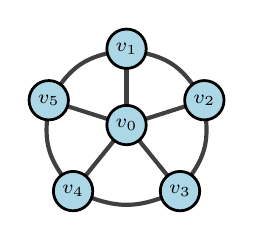
\begin{tikzpicture}
            \Vertex[x=0, y=0.904, size=0.5, label=$v_1$]{A}
            \Vertex[x=0.988, y=0.25, size=0.5, label=$v_2$]{B}
            \Vertex[x=0.679, y=-0.904, size=0.5, label=$v_3$]{C}
            \Vertex[x=-0.679, y=-0.904, size=0.5, label=$v_4$]{D}
            \Vertex[x=-0.988, y=0.25, size=0.5, label=$v_5$]{E}
            \Vertex[y=-0.065,size=0.5, label=$v_0$]{Z}
            \Edge[bend=20](A)(B)
            \Edge[bend=20](B)(C)
            \Edge[bend=20](C)(D)
            \Edge[bend=20](D)(E)
            \Edge[bend=20](E)(A)
            \Edge(Z)(A)
            \Edge(Z)(B)
            \Edge(Z)(C)
            \Edge(Z)(D)
            \Edge(Z)(E)
        \end{tikzpicture}
    \end{figure}
\end{document}